\documentclass[11pt, oneside]{article}   	% use "amsart" instead of "article" for AMSLaTeX format
\usepackage{geometry}                		% See geometry.pdf to learn the layout options. There are lots.
\geometry{letterpaper}                   		% ... or a4paper or a5paper or ... 
%\geometry{landscape}                		% Activate for for rotated page geometry
%\usepackage[parfill]{parskip}    		% Activate to begin paragraphs with an empty line rather than an indent
\usepackage{graphicx}				% Use pdf, png, jpg, or eps§ with pdflatex; use eps in DVI mode
								% TeX will automatically convert eps --> pdf in pdflatex		
\usepackage{amsmath, amssymb}    % May not all be necessary
\usepackage{graphicx}                    % For including pictures
\usepackage{hyperref}                    % For formatting (clickable) URLs
\usepackage{algpseudocode}
\usepackage{algorithm}
\usepackage{mfirstuc}
\usepackage{graphicx}
\usepackage{amsopn}
\usepackage{url}
\usepackage{parskip}
\usepackage{wrapfig}
\usepackage{color}
\usepackage[usenames,dvipsnames,svgnames,table]{xcolor}
\usepackage{grffile}
\usepackage{comment}
\usepackage{epsfig}
\usepackage{float}
\usepackage{subfigure}
\usepackage{verbatim}
\usepackage{multirow}
\usepackage{todonotes}
\usepackage{epstopdf}
\usepackage{amssymb}
\usepackage{multirow}
\usepackage{hhline}

\presetkeys{todonotes}{inline}{}

\newcommand\figref{Fig.~\ref}
\newcommand\secref{Section~\ref}
\newcommand\tabref{Table~\ref}

\title{CS 659 Course Project \\ Restaurant Revenue Prediction}
\author{Huangxin Wang and Zhonghua Xi \\
\\
Computer Science Dept. \\
George Mason University}
%\date{}							% Activate to display a given date or no date

\begin{document}
\maketitle

\section{Introduction}
\todo{re-phrase this section}
Deciding when and where to open new restaurants is largely a subjective process based on the personal judgement and experience of development teams. 
This subjective data is difficult to accurately extrapolate across geographies and cultures.
New restaurant sites take large investments of time and capital to get up and running. 
When the wrong location for a restaurant brand is chosen, the site closes within 18 months and operating losses are incurred. 
Finding a mathematical model to increase the effectiveness of investments in new restaurant sites would allow funds to invest more in other important business areas, like sustainability, innovation, and training for new employees.
The goal of this project is to predict the revenues of restaurants by given demographic, real estate, and commercial data of existing restaurants withe their current revenues.

%\subsection{}
\section{Dataset}
We collect the data from Kaggle, a community of data scientists which also hosts competitions. 
Restaurant revenue prediction is one of the active competition.
There are 137 restaurants in the training set and 100000 in the test set which is an unbalanced dataset. 
For each record, 41 features are given detailed in \tabref{tab:features}.

\begin{table}[htdp]
\footnotesize
\caption{Features}
\begin{center}
\begin{tabular}{|r|l|}
\hline
\bf{Name} 		& \bf{Description} \\ \hline
\bf{Open Date}	& Categorical. Opening date for a restaurant. \\ \hline
\bf{City}		& Categorical. City that the restaurant is in. \\ \hline
\bf{City Group} & Categorical. Type of the city. Big cities, or Other. \\ \hline
\bf{Type}		& \begin{tabular}{@{}l@{}} Categorical. Type of the restaurant. \\ FC: Food Court, IL: Inline, DT: Drive Thru, MB: Mobile. \end{tabular}   \\ \hline
\bf{P1-P37}		& \begin{tabular}{@{}l@{}} Numerical. Three categories of these obfuscated data. \\ 
\bf{Demographic data} \\
Gathered from third party providers with GIS systems. \\ 
These include population in any given area, age and \\
gender distribution, development scales. \\
\bf{Real estate data} \\
Mainly relate to the m2 of the location, front facade \\
of the location, car park availability. \\
\bf{Commercial data} \\
Mainly include the existence of points of interest \\
including schools, banks, other QSR operators. \end{tabular}   \\ \hline
\bf{Revenue}	& \begin{tabular}{@{}l@{}} A transformed revenue of the restaurant in a given year \\
Only provided in training set.
\end{tabular} \\ \hline
\end{tabular}
\end{center}
\label{tab:features}
\end{table}%

\subsection{Data Preparation}
\subsubsection{Revenue at a Glance}
In \figref{fig:revenue} we show the histogram of the revenues, from which we can see majority of the revenues are around $5 \times 10^6$, 
however, there are few ``outliers'' which makes both training and prediction hard especially under RMSE evaluation metric.

\begin{figure}[htbp] %  figure placement: here, top, bottom, or page
   \centering
   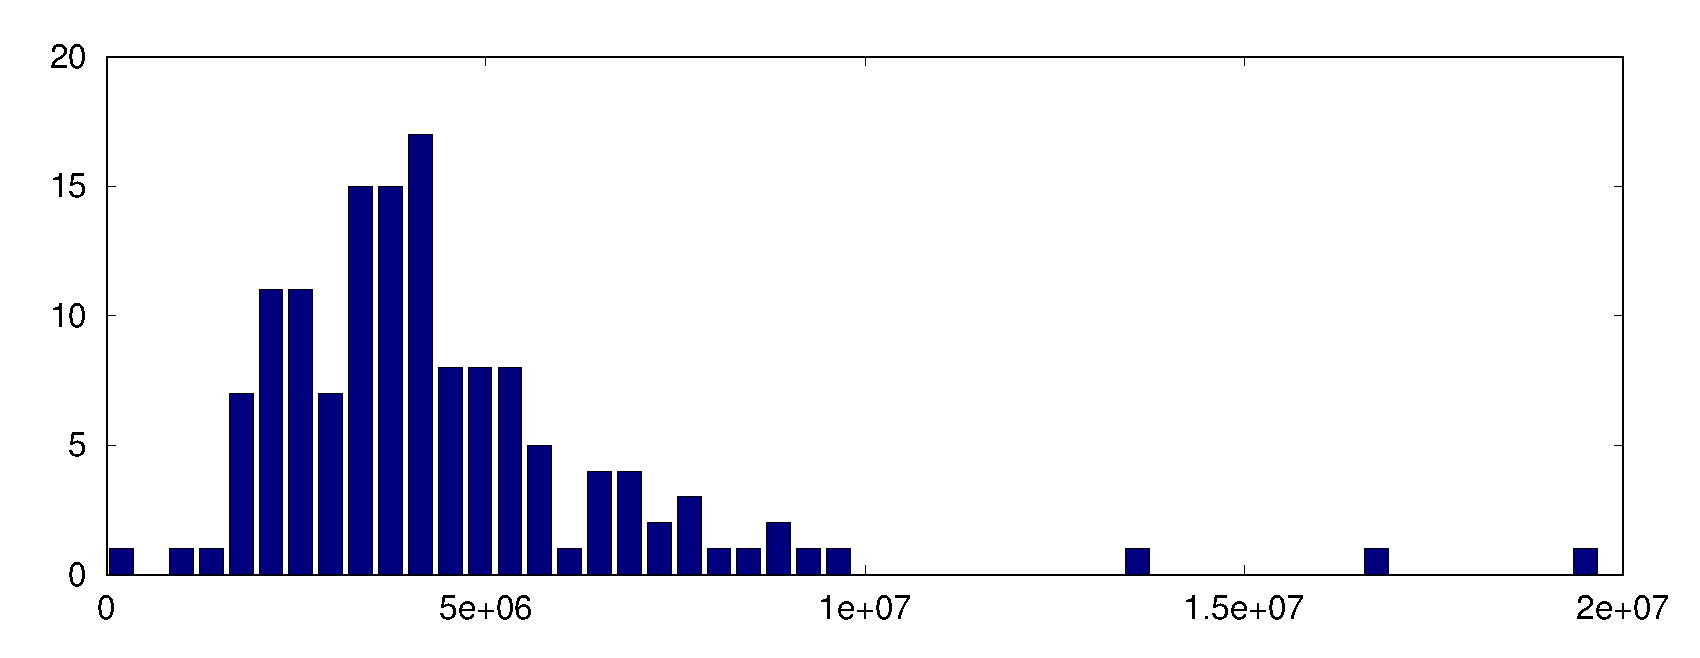
\includegraphics[width=5in]{figs/revenue.eps} 
   \caption{Histogram of revenues.}
   \label{fig:revenue}
\end{figure}

\subsubsection{Features Selection}

{\bf Missing Categories} 
After a quick exploration of both training set and test set we found that both {\bf City} and {\bf Type} features have unseen categories in the training set.
There are total 63 cities in the entire dataset, too many new features will be added if we create a binary feature for each city and 
the there is no correlation between these two features and revenue.
Thus we decided to drop both {\bf City} and {\bf Type} features.

\subsubsection{Feature Normalization}

\section{Methodology}
\section{Results and Discussion}
\section{Conclusion}


\end{document}  